\documentclass[11pt,letterpaper,dvipsnames]{article}
%\usepackage{fullpage}
\usepackage{multicol}
\usepackage{amsmath}
\usepackage{amsfonts}
\usepackage{amssymb}
\usepackage{amsthm}
\usepackage{hyperref}
\usepackage{graphicx, nicefrac}
\usepackage{tikz, nicefrac}

\DeclareMathAlphabet\EuScript{U}{eus}{m}{n}
\SetMathAlphabet\EuScript{bold}{U}{eus}{b}{n}

\linespread{1.15}

\newenvironment{solution}{\color{SeaGreen}\textit{Solution.}}{\color{black}}

\theoremstyle{definition}
\newtheorem{definition}{Definition}[section]
\newtheorem{example}{Example}[section]
\newtheorem{theorem}{Theorem}[section]
\newtheorem{corollary}{Corollary}[theorem]
\newtheorem{lemma}[theorem]{Lemma}

\newcommand{\ds}{\displaystyle}
\newcommand{\bv}{\mathbf}
\newcommand{\lv}{\langle}
\newcommand{\rv}{\rangle}
\newcommand{\bb}[1]{\mathbb{#1}}
\newcommand{\es}[1]{\EuScript{#1}}

\title{\textbf{Combinatorics in Education:\\ An Introduction to Knowledge Space Theory}}
\author{Carson Mulvey}
\date{MAD4204}

\begin{document}

\maketitle

\section*{Introduction} %TODO Update "motivation"

The goal of this project is to give an introductory overview to the theory of knowledge and learning spaces, a field that mixes combinatorics and mathematical psychology. We will cover some principles of knowledge and learning spaces and demonstrate algorithmic solutions to creating these spaces. We will also show the connections between knowledge space theory and the content from our course. Learning spaces in particular closely tie into poset and lattice theory, and as such, the knowledge from course content relating to posets is assumed. The active component of the project is an implementation one of the explained algorithms. The source code is available on GitHub
\footnote{\href{https://gist.github.com/heyuncle/94b858fdbb9a256d424766b361e6c283}{https://gist.github.com/heyuncle/94b858fdbb9a256d424766b361e6c283}} 
and a demonstration is available on YouTube
\footnote{\href{https://youtu.be/gebNB3qwiBQ}{https://youtu.be/gebNB3qwiBQ}}.

The theory of knowledge spaces is relatively new, beginning with a joint paper between Doignon and Falmagne (1985). The field uses a combinatorial approach to assessing competency in a skill, attempting to create more informative psychometric measures than the singular numbers produced by assessments such as the SAT and ACT. Since then, the field has been extensively researched and applied by the popular website \textbf{A}ssessment and \textbf{LE}arning in \textbf{K}nowledge \textbf{S}paces, better known as ALEKS, to develop an online platform for learning math and chemistry. The theory of knowledge spaces is still currently researched and applied to online platforms like ALEKS to more effectively teach and measure skill levels in various school subjects.


\section{Knowledge Space Theory}

Suppose that as a teacher, we want to measure a student's ability in a subject. To have a detailed understanding of what the student does or doesn't understand, we split a subject into a set of distinct `skills' $Q$. Then for some $K\subseteq Q$, we can think of $K$ as the skills that a students already knows. The empty set and $Q$ itself are clearly possibilities for $K$, representing the student knowing nothing or everything about the subject, respectively. However, not all $K$ are necessarily \textit{feasible} subsets of skills a student can have, leading to our first definition.

\begin{definition}
    The pair $(Q,\EuScript{K})$ is a \textit{knowledge structure}, given nonempty set $Q$ and family $\EuScript{K}\subseteq 2^Q$ containing $Q$ and $\varnothing$. We call $Q$ the \textit{domain} and $\EuScript{K}$ the \textit{(knowledge) states} of the knowledge space.
\end{definition}

Note that because $\bigcup_{K\in\EuScript{K}}K=Q$, we may denote a knowledge structure by just $\EuScript{K}$ without causing any ambiguity.

Also, we often use $\es{K}_q$ for some $q\in Q$ to denote the subset of $\es{K}_q$ of all knowledge states containing $q$.

\begin{example}
    Consider the domain $Q=\{a,b,c,d\}$ with knowledge states
    \[
        \EuScript{K} = \{\varnothing,\{a\},\{b\},\{a,b\},\{a,c\},\{a,d\},\{a,b,c\},\{a,b,d\},\{a,c,d\},Q\}.
    \]
    We see that $(Q,\EuScript{K})$ is indeed a knowledge structure, as all subsets $K\in\EuScript{K}$ are in the power set of $Q$, with both $\varnothing$ and $Q$ itself in $\EuScript{K}$.
\end{example}

However, this definition alone is very loose; an arbitrary subset of skills $K$ on its own encodes very little pedagogical information. As such, we add restrictions that lead to the \textit{knowledge spaces} and \textit{learning spaces} that make up the majority of the theory.

\begin{definition}
    A knowledge structure $(Q, \es{K})$ (also commonly notated as $\es{K}$) is called a \textit{knowledge space} if it is \textit{union-closed}, i.e. if for all $A,B\in\es{F} \subseteq \es{K}$, we have $A\cup B \in \es{F}$.

    A \textit{quasi-ordinal knowledge space} is a knowledge space $\es{K}$ with the additional restriction of being \textit{intersection-closed}, i.e. if for all $A,B\in\es{F} \subseteq \es{K}$, we have $A\cap B \in \es{F}$.
\end{definition}


Knowledge spaces, as opposed to knowledge structures, add a meaningful restriction in terms of pedagogical interpretation. They can be interpreted as the existence of an expert on a topic in a class allowing for all students to eventually master that topic as well. Additionally, a quasi-ordinal knowledge structure has the additional property that if one student knows skills $a$ and $b$, and another student knows skills $b$ and $c$, then a third student may only know skill $b$.

\begin{definition}
A \textit{well-graded knowledge space} is a knowledge space $\es{K}$ satisfying the additional axiom:
\begin{enumerate}
    \item[(MA)] For nonempty $K\in \es{K}$, there exists some $q$ in $K$ such that $K \setminus \{q\}\in \es{K}$.
\end{enumerate}
\end{definition}

Well-graded knowledge spaces allow us to create a `tight path' between two knowledge states, i.e. a sequence $K=K_0,K_1,\dots,K_p=L$ where $|A\triangle B|=1$ for $i\in[p]$. Also, a union-closed family satisfying the (MA) axiom may also be referred to as an \textit{antimatroid}.

Finally, we define a very special case of a knowledge space called a learning space.

\begin{definition}
    A knowledge structure $(Q, \es{K})$ is a \textit{learning space} if it satisfies the following axioms:
    \begin{enumerate}
        \item[(L1)] For any two states $K$ and $L$ with $K\subset L$, there exists a finite chain
        \[
            K=K_0\subset K_1\subset \cdots K_p=L
        \]
        with $|K_i\setminus K_{i-1}|=1$ for $i\in [p]$.
        \item[(L2)] For any two states $K$ and $L$ with $K\subset L$, if some $q$ satisfies $K+\{q\}\in \es{K}$, then $L\cup \{q\}\in \es{K}$.
    \end{enumerate}
\end{definition}

Axiom (L1) can be interpreted as the ability to go between knowledge states by learning skills one at a time. Axiom (L2), on the other hand, shows that a learner can continue learning even at a greater knowledge state.

Finally, the following result connects these varieties of knowledge structures together.

\begin{theorem}
    For a knowledge structure $(Q,K)$, the following statements are equivalent:
    \begin{enumerate}
        \item (Q, K) is a learning space. 
        \item (Q, K) is a well-graded knowledge space.
    \end{enumerate}
\end{theorem}




% In the theory of knowledge spaces, we represent a subject $S$ as a set of ``skills'' or ``problems'' $Q$ that make up that field. Taking some partial order $\leq$ on $Q$ gives a poset $(Q,\leq$).

% However, this model isn't necessarily accurate to skills being learned, as there isn't always a defined order to learn certain skills. The first restriction we relax on our setup is the \textit{antisymmetric} condition of the partial order. A reflexive and transitive, but not necessarily antisymmetric relation is called a \textit{quasi-order}. An example is shown in Figure 2.

% \begin{figure}[h]
%     \centering
%     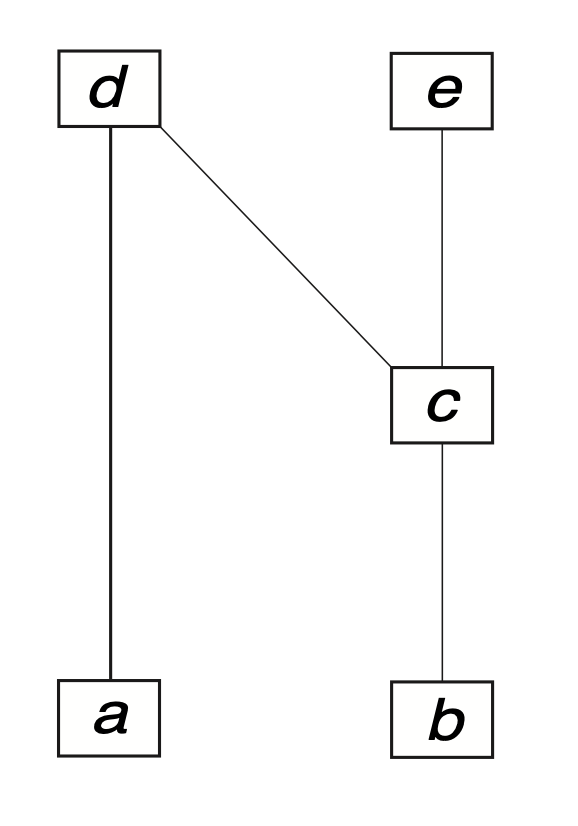
\includegraphics[width=0.2\columnwidth]{poset.png}
%     \caption{Example poset on $Q=[5]$.}
% \end{figure}

% \begin{figure}[h]
%     \centering
%     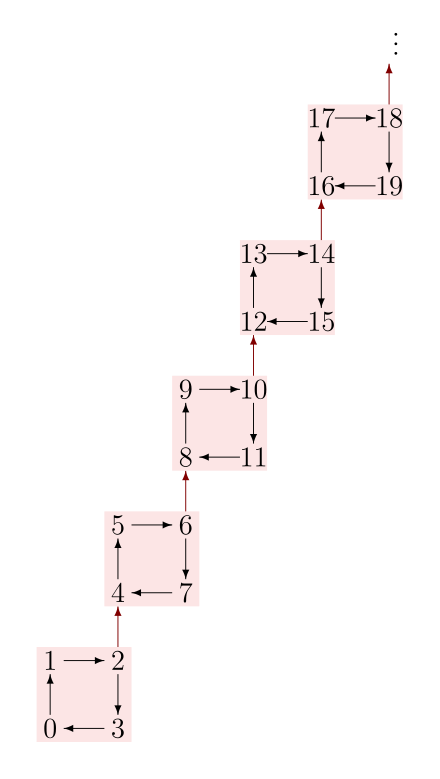
\includegraphics[width=0.2\columnwidth]{qoset.png}
%     \caption{Example of a quasi-order.}
% \end{figure}

% \section{Birkhoff's Representation Theorem, Revisited}

% There may be a striking resemblance between the definitions made so far and the theory of posets and lattices that we covered in class. This is no mistake, as there are close ties and applications of lattice theory within knowledge space theory.


% \begin{definition}
%     Let $(Q,\es{K})$ be a knowledge structure. Then we define the \textit{surmise relation} $\precsim$ on $Q$ by
%     \[
%         r\precsim q \iff r\in \bigcap_{K\in\es{K}} \es{K}_q.
%     \]
% \end{definition}


%Notes
% Antimatroid = Learning space = Well graded knowledge space (prove?)
% Example of Antimatroid: J(P)


\section{Building Knowledge Spaces: \\Naive \texttt{QUERY} Algorithm}

In the context of knowledge spaces, we often want to create a knowledge space by finding the feasible knowledge states for a particular subject. However, to make these states accurate, we must find a heuristic that will let us determine when a state is \textbf{not} feasible. As such, we create the following query:

\begin{enumerate}
    \item[(Q1)] Suppose that a student has failed to solve all items in a nonempty subset $A$ of domain $Q$. Do you believe this student would also fail to solve item $q$? You may assume that chance factors, such as lucky guesses and careless errors, do not interfere in the student's performance.
\end{enumerate}

This query was developed for the \texttt{QUERY} algorithm, an algorithm developed by Koppen in 1993. We will show the process of a simplified version of \texttt{QUERY}, known by Doignon and Falmagne as `a naive querying algorithm'.

First, we will define a relevant relation, an `entailment' for a domain $Q$.

\begin{definition}
    An \textit{entailment} for a domain $Q$ is a relation $\es{P}$ from $2^Q\setminus\{\varnothing\}$ to $Q$ satisfying
    \[
        A\es{P}q \iff (\forall K\in \es{K} : A \cap K = \varnothing \Rightarrow q \notin K).
    \]
    An entailment on $Q$ satisfies the following properties:
    \begin{enumerate}
        \item[(i)] If $q\in A\subseteq Q$, then $A\es{P}q$.
        \item[(ii)] If $A,B\in 2^Q\setminus\{\varnothing\}$ and $q\in Q$, then $A\es{P}b$ for all $b\in B$ and $B\es{P}p$ imply $A\es{P}p$.
    \end{enumerate}
\end{definition}

Most importantly, a theorem from Doignon and Falmagne is used to connect membership in an entailment and feasible states in a knowledge space.

\begin{theorem}
    There is a one-to-one correspondence between the family of all knowledge spaces $K$ on the same domain $Q$, and the family of all entailments $\es{P}$ for $Q$. This correspondence is defined by the two equivalences
    \begin{align}
        A \es{P} q &\iff (\forall K\in \es{K} : A \cap K = \varnothing \Rightarrow q \notin K), \\
        K\in \es{K} &\iff (\forall(A,p)\in\es{P}: A \cap K = \varnothing \Rightarrow p \notin K).
    \end{align}
\end{theorem}

Using (2) from this equivalence lets us design the following algorithm:

\begin{enumerate}
    \item[Step 1.] Draw up the list of all the subsets of $Q$.
    \item[Step 2.] Successively submit all the queries $(A, q)$ of the form [Q1]. Whenever a positive response $A\es{P}q$ is observed, remove from the list of remaining subsets all the sets containing $q$ and disjoint from $A$.
\end{enumerate}

If all queries are submitted, then (2) shows exactly which subsets $K$ are or are not in $\es{K}$, hence showing the exact knowledge space $\es{K}$.


%\subsection{Knowledge state assessment} % TODO ?



% \section{Bibliography} % TODO bibtex
% \begin{enumerate}
%     \item Jean-Paul Doignon, Jean-Claude Falmagne (2015). "Knowledge Spaces and Learning Spaces". arXiv:1511.06757
%     \item Doignon, J.-P.; Falmagne, J.-Cl. (1999), Knowledge Spaces, Springer-Verlag, ISBN 978-3-540-64501-6.
%     \item Falmagne, J.-Cl.; Albert, D.; Doble, C.; Eppstein, D.; Hu, X. (2013), Knowledge Spaces. Applications in Education, Springer.
%     \item Schrepp, M. (1999), "Extracting knowledge structures from observed data", British Journal of Mathematical and Statistical Psychology, 52 (2): 213–224, doi:10.1348/000711099159071
%     \item Cosyn, E., and Uzun, H.B. 2009. Note on two necessary and sufficient axioms for a well-graded knowledge space. Journal of Mathematical Psychology, 53, 40–42.
%     \item Korte, Bernhard; Lovász, László; Schrader, Rainer (1991), Greedoids, Springer-Verlag, pp. 19–43, ISBN 3-540-18190-3
%     \item Boyd, E. Andrew; Faigle, Ulrich (1990), "An algorithmic characterization of antimatroids", Discrete Applied Mathematics, 28 (3): 197–205, doi:10.1016/0166-218X(90)90002-T
% \end{enumerate}

\end{document}